\label{sec:EfficientElectronicStructure}
\subsubsection{Molecular Symmetry}
Electronic structure calculations are performed at a fixed molecular geometry, and thus it is useful to define orbitals that transform in a well defined fashion with the Hamiltonian. Molecular orbitals transform as irreducible representations within the molecule's point group, a closed set of symmetry operations under which the molecule remains unchanged. A visual example, the pi system of benzene, is comprised of four irreducible representations within the $D_{6h}$ point group. $\Gamma_{\pi} = \Gamma_{A_{2u}} + \Gamma_{E_{1g}} + \Gamma_{E_{2u}} + \Gamma_{B_{2g}} \in D_{6h}$
\begin{figure}[H]
	\centering
	\begin{tabular}[m]{m{0.2\textwidth} m{0.2\textwidth}m{0.2\textwidth}p{0.2\textwidth}}
		\multirow{2}*{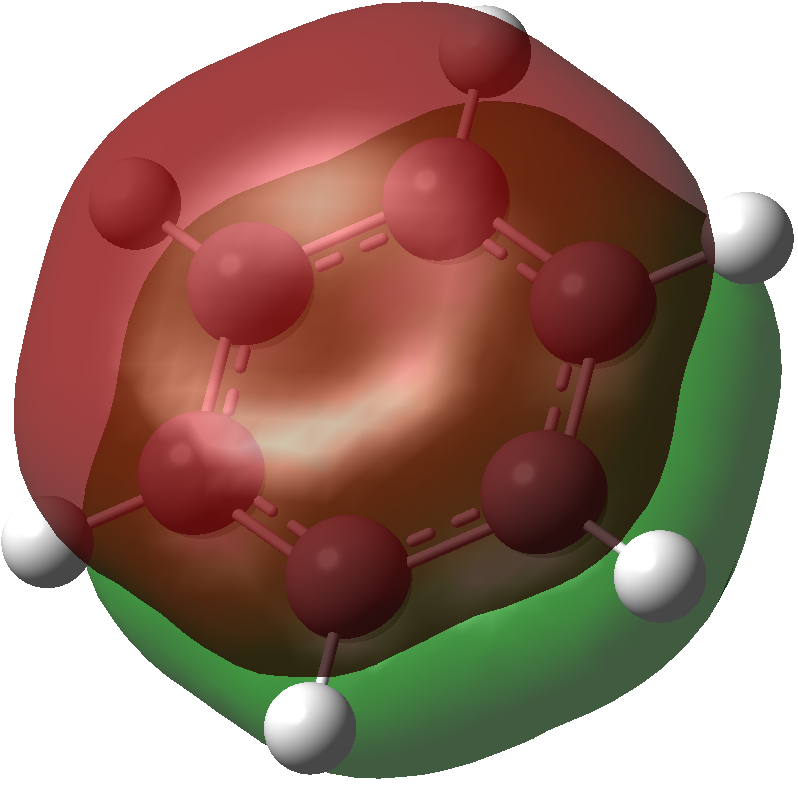
\includegraphics[width=0.15\textwidth]{images/BenA2u.png}} 
	 	&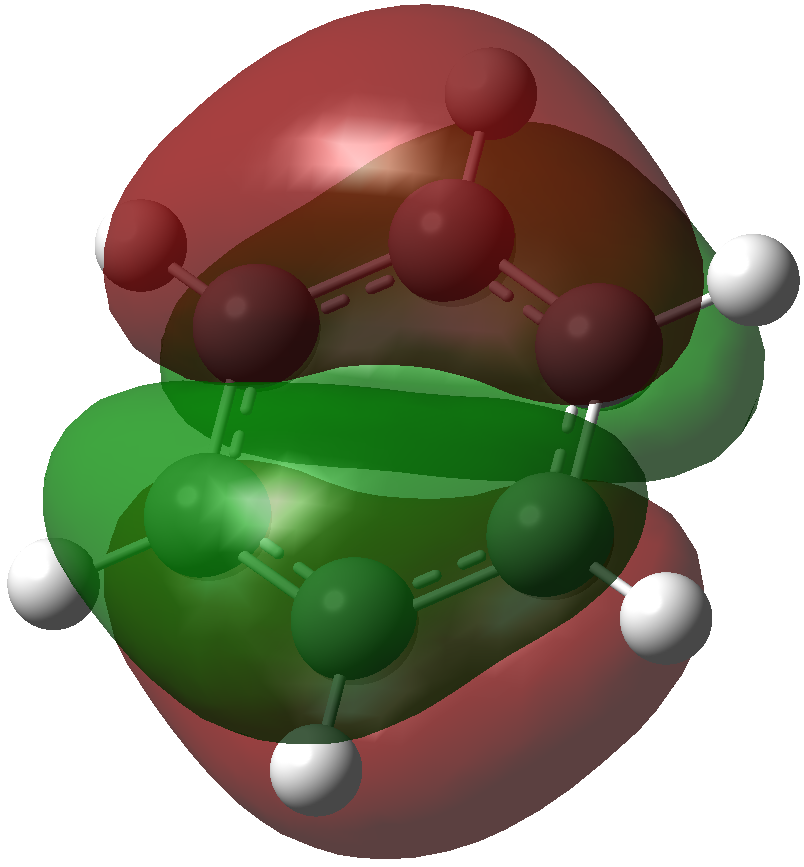
\includegraphics[width=0.15\textwidth]{images/BenE1g1.png}
	 	&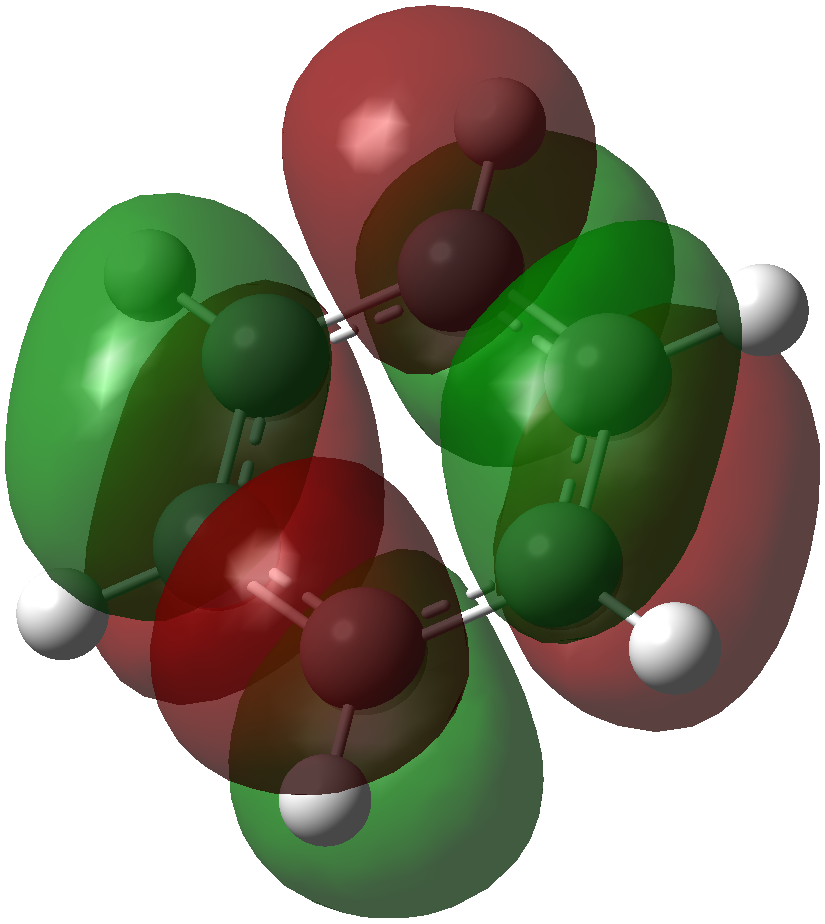
\includegraphics[width=0.15\textwidth]{images/BenE2u1.png}
	 	&\multirow{2}*{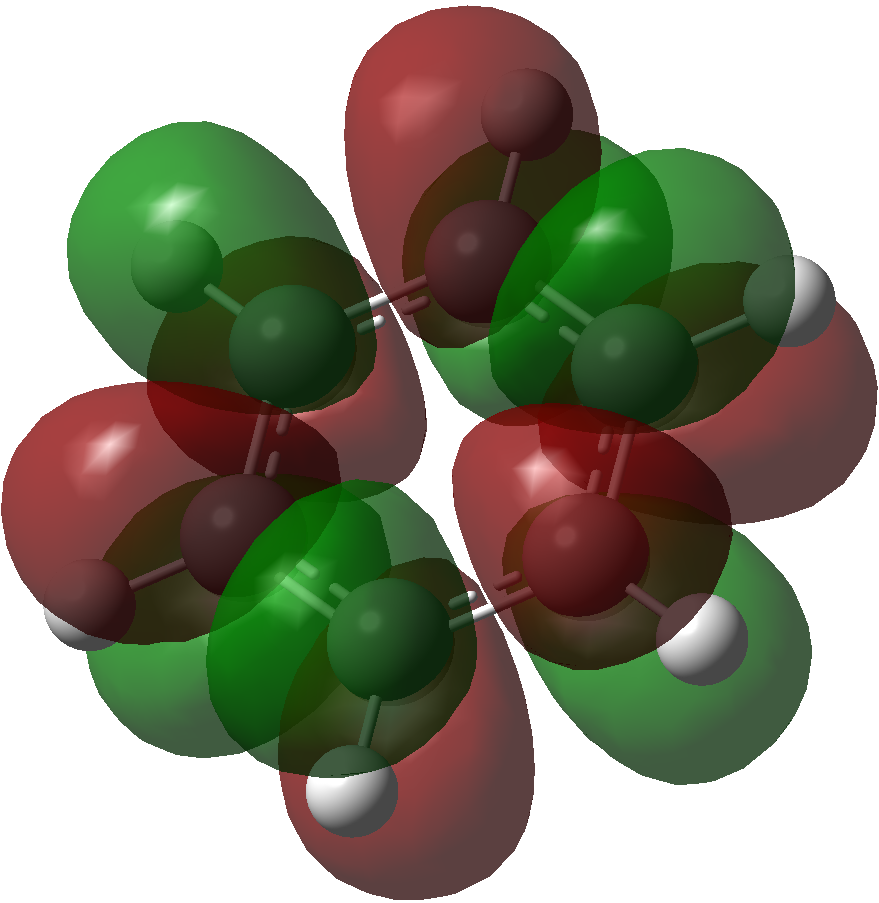
\includegraphics[width=0.15\textwidth]{images/BenB2g.png}} \\
		&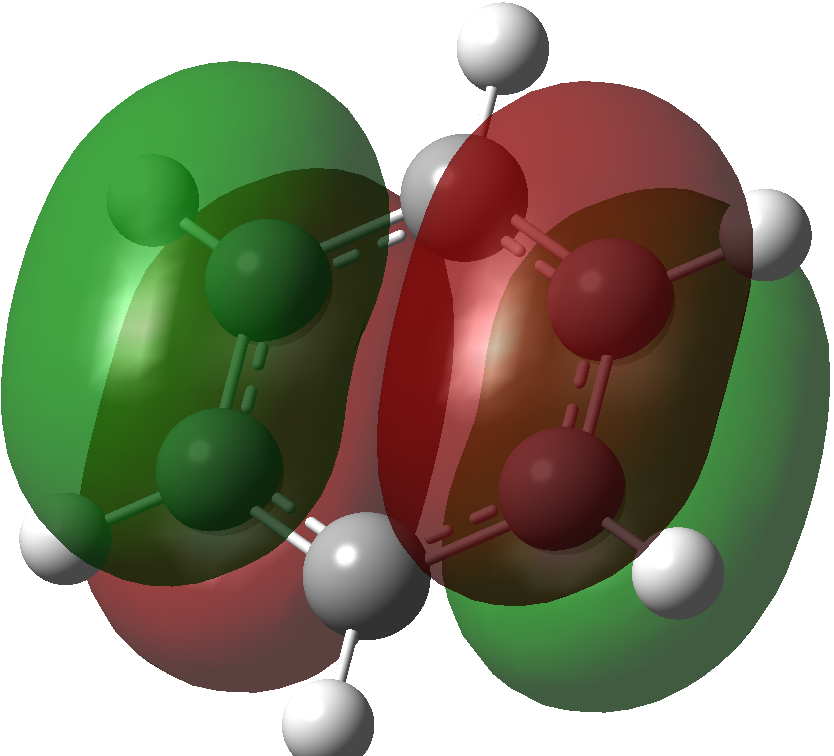
\includegraphics[width=0.15\textwidth]{images/BenE1g2.png}
		&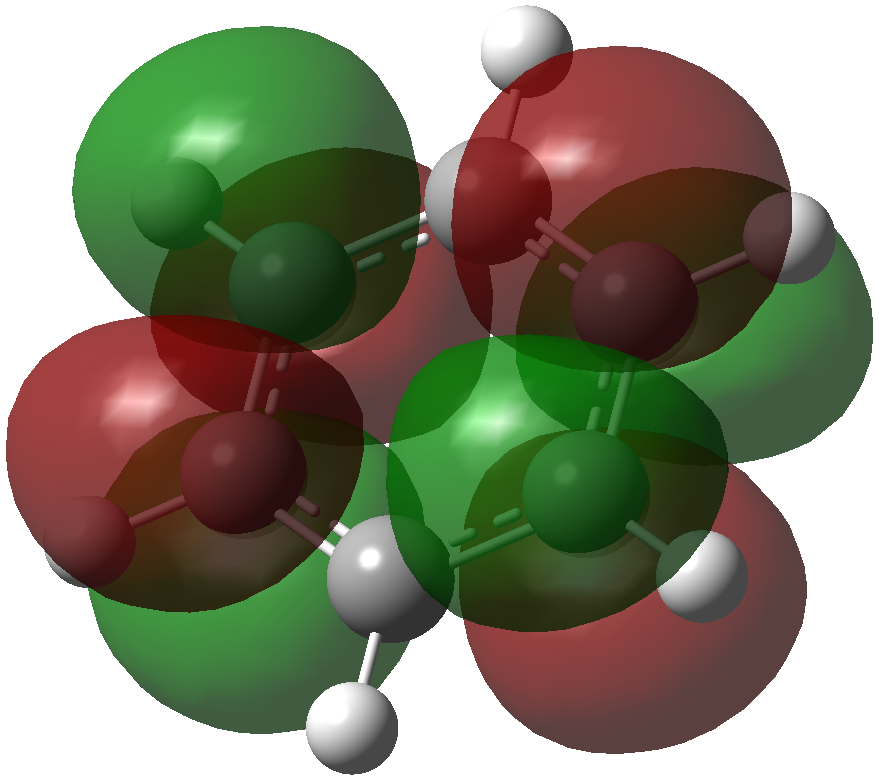
\includegraphics[width=0.15\textwidth]{images/BenE2u2.png}\\	
		\centering $A_{2u}$ &
		\centering $E_{1g}$ &
		\centering  $E_{2u}$ &
		\centering $B_{2g}$  \\
	\end{tabular}
	\caption{Canonical $\pi$ orbitals of benzene}
\label{fig:pirep}
\end{figure}
Rather than describe a specific arrangement of atoms, point groups are an abstraction of the number of ways an object be symmetric, much the same way the number two is an abstraction of any pair of objects. In the context of coupled cluster, integrals and t-amplitudes are heavily constrained by symmetry, e.g. a t-amplitude is zero unless the product of its orbital's irreducible representations is $A_1$.
\begin{align}
\Gamma_a \otimes \Gamma_i \otimes \dots  = A_1 + \dots
\end{align}
This fact is leveraged by organizing MOs into blocks of symmetry, where only products of orbitals in the same symmetric block are considered, the resulting matrix of t-amplitudes are is block diagonal:
\begin{equation*}
\hat{T}_{n}=\begin{array}{c| c c c c c}
&A_1 & \Gamma_2 & \cdots & \Gamma_n\\
\hline
A_1 & X_{11} &0 & \cdots & 0\\
\Gamma_2  & 0 & X_{22} &\cdots&0\\
\vdots & \vdots &\vdots & \ddots & 0\\
\Gamma_n & 0&0 & \cdots & X_{nn}
\end{array}\label{eq:diag}
\end{equation*}
This partitioning reduces the computational cost by a constant factor of $h^2$, where h is the number of irreducible representations. However, because the resulting MO's are de-localized over the the entire molecule, computational effort increases exponentially. Currently, methods involving localized orbitals are of particular interest 
\subsection{Local Correlation Theory}

\subsubsection{Overview}
The harsh scaling of CC methods largely stems from the delocalized character of the canonical orbitals \cite{DLPNOCC,MP2}. As electrons are added to the system, the number of correlated electron pairs increases quadratically, while the number of strongly-correlated electron pairs grows linearly. The computational complexity is dominated by weakly interacting pairs, whose interaction falls with $R^{-6}$. These interactions cannot be ignored, however calculations involving highly localized orbitals with an approximate treatment of long-range forces have shown to give accurate results while scaling like DFT. Two methods of particular interest are domain-based local pair natural orbital (DLPNO), and cluster-in-molecule (CIM). DLPNO solves the canonical equations under a local approximation, while CIM divides the system into fragments and indirectly assembles the energy from many parallel calculations. Both methods are commonly implemented in conjunction with perturbation theory. Currently, work is ongoing to combine these methods. The correlation energy can be written 
\begin{equation}
E^{cor} = \sum_{ijab} \bigg( 2 \braket{ij|ab} - \braket{ij|ba}\bigg) \tau^{ab}_{ij} \label{eq:e_corr}
\end{equation}
individual t-amplitudes $\tau^{ab}_{ij}$ can be calculated at either the CC or MP2 level: 
\begin{equation}
\tau_{ij}^{ab} =
\begin{cases}
t_{ij}^{ab} + t_i^a t_j^b -t_i^b t_j^a  ,&(CCSD)\\
t_{ij}^{ab}, &(MP)
\end{cases}
\end{equation}
\cref{eq:e_corr} is invariant under orbital rotations, and is valid in both the canonical and localized representation. Efficient partitioning of this summation is a convenient basis of discussion for local methods.

The first local correlation method was develoepd by Pulay et. al. in 1983, wherein MPPT calculations were performed using orthogonal localized molecular orbitals (LMO's) and nonorthongonal projected atomic orbitals (PAO) for the occupied and virtual space, respectively \cite{PULAY1983151}. The local schema demonstrated that $>98\%$ of the correlation energy can be recovered via the use of a unique, local, domain in addition to an approximate treatment of long-range effects \cite{doi:10.1063/1.454111,SAEBO198513,doi:10.1146/annurev.pc.44.100193.001241}. This approach was further refined by Werner and Schütz, who generalized the method for use in coupled-cluster type calculations  \cite{doi:10.1063/1.471289, doi:10.1063/1.1330207,doi:10.1063/1.3696963,doi:10.1063/1.3641642}.

\subsubsection{DLPNO-CC}
  This method was further refined by constructing approximate natural orbitals specific to each electron pair. CI calculations involving two-electron systems rapidly converge when utilizing NO's ordered by decreasing occupation number \cite{PhysRev.97.1474}. LPNO domains grow slowly with respect to basis size, and help prevent the local domains from becoming prohibitively large. \cite{MEYER, LPNOCC}.  DLPNO carries out \cref{eq:e_corr} over the virtuals $a,b$. The resulting equation expresses the correlation energy as a sum over all electron pairs: 
\begin{equation}
E^{cor} = \sum_{ij}E^{corr}_{ij} = \sum_{ij} \sum_{ab}  \bigg( 2 \braket{ij|ab} - \braket{ij|ba}\bigg) \tau^{ab}_{ij}
\end{equation}
The number of pairs scales quadratically with the system size, but the contributions from a large percentage of pairs are negligible. Each electron pair is associated with a virtual space of constant size. The pairs are pre-screened, and weakly interacting pairs may be discarded. Surviving amplitudes are coupled and can be determined with CC or MP2, depending on their expected interaction strength. For large systems, this pre-screening reduces the number of t-amplitudes to be calculated by a factor of roughly $10^5$, while retaining $> 99.5\%$ of the correlation energy \cite{DLPNOCC}. As a result, LPNO scales linearly for systems of containing less than 80 atoms. For larger systems, the improved domain-based LPNO  technique is applicable.  At the time of its publication, Neese et. al. showed successful DLPNO treatment for systems typically outside the reach of canonical CC or even LPNO-CC (Figure \ref{vanco}). In their implementation, less than 10\% of all electron pairs were given full-accuracy treatment. The canonical CC equations are modified under DLPNO, and, if not properly implemented, the associated integral transformations can up the majority of the DLPNO runtime. Existing, optimized CC code is incompatible with DLPNO. As a result, new DLPNO implementations require a considerable effort.
\begin{figure}[H]
\centering
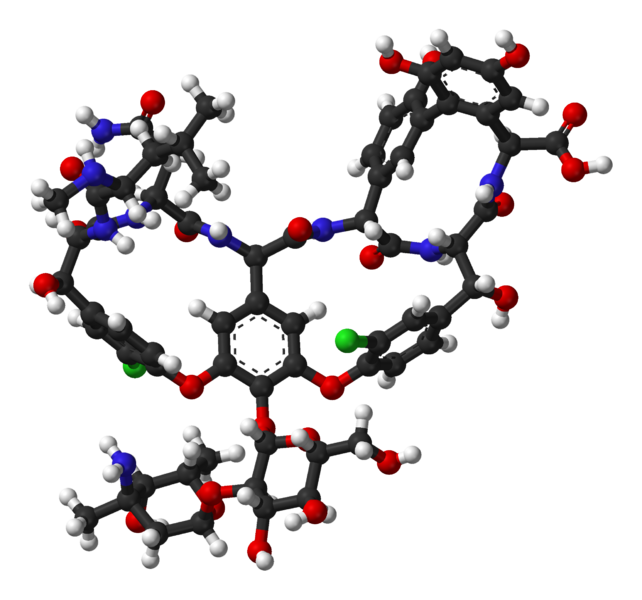
\includegraphics[scale=0.35]{images/Vanco.png}
\caption{Chemical structure of vancomycin: 176 atoms, 3593 basis functions (def2-TZVP)}
\label{vanco}
\end{figure}
\subsubsection{Cluster in Molecule}
In contrast to the 'direct' nature of DLPNO, the 'fragment' based CIM schema divides the system into a number of localized clusters. Each occupied orbital is assigned a subset of orbitals, $P_i$, which, by some measure, interact strongly with the central orbital, $i$. The correlation energy is taken to be a sum over the clusters, and thus \cref{eq:e_corr} is carried out over a single occupied orbital index:
\begin{equation}
E^{cor} =\sum_i^{N_{occ}} E^{corr}_{i} = \sum_{i} \sum_{jab} \bigg( 2 \braket{ij|ab} - \braket{ij|ba}\bigg) \tau^{ab}_{ij}
\end{equation}

There are three important advantages of CIM that should be kept in mind; parallelization, the multi-level extension and compatibility with existing code.
\begin{description}
\item[Parallelization] The CC equations only need to be solved for a series of clusters, instead of for the system as a whole. As these calculations can be carried out in parallel, the overall scaling of CIM depends only on the largest cluster size. In addition, the size of the clusters, is independent on the overall system-size \cite{doi:10.1080/00268976.2016.1139755}. The memory and disk requirements are also constant
\item[Multi-level CIM] Multi-level CIM allows different clusters to be treated with varying levels of theory.  Chemically important motifs can be treated with a high-accuracy method, while atoms far from a reaction center can be treated with a more efficient low-accuracy method. The mixed-accuracy energy is still the sum over all clusters: 
\begin{equation}
E^{corr} = \sum_{i \in P} E^{CCSD}_i + \sum_{j \in Q} E^{MP2}_j
\end{equation}
Where $P$ and $Q$ are clusters which are to be treated with e.g. CCSD and MP2, respectively.
This concept of mixed-accuracy techniques will be later discussed in context of our ground-state method.
\item[Compatibility] Once the clusters are defined, it is possible to use existing canonical CC code with CIM. This is ease of implementation is the exception rather than the norm. As it stands, a CIM implementation using CCSDTQ code could be developed with a moderate development overhead. 

\end{description}
Despite its advantages, CIM is not without faults. The efficiency of the CIM technique is strongly dependant on the size of the clusters, and also the manner in which the clusters are constructed. Canonical CC calculations are carried out on each individual cluster, and if generous thresholds are chosen to ensure accurate results, the resulting clusters may be too large to reasonably treat. Going too far in the other direction, clusters may be too small to yield accurate energies. It is clear the construction of clusters must be done with some level of care. As it is our hope that our work contributes positively to this problem, and as such the major steps of CIM cluster construction are outlined below: 
\begin{enumerate}
\item Localized occupied orbitals are generated via some procedure. Foster-Boys was initially used, but scales as $\mathcal{O}(N^3)$. Pipek-Mezey or natural localized orbitals have also been implemented \cite{doi:10.1063/1.3641642}. 
\item Each occupied LMO $i$ is assigned to an atom with the greatest Mulliken atomic charge. This atom is the 'central atom' of the LMO. \item For a given LMO $i$, LMOs which interact strongly with the central orbital are added to the MO domain. Originally, distance thresholds were used, but methods which do not utilize real-space cut-offs have also been developed. In such cases quantities such as differential overlap integrals are used. 
\item If any domains are completely enveloped by larger domains, they are combined. Thus a single $P_i$ may consist of multiple LMO's and the overall number of clusters is reduced. 
\item For each LMO in a given domain, an AO domain is constructed in a similar manner to the MO domains. 
\item The occupied LMOs of a cluster $P_i$ are taken to be the LMOs projected onto the final AO domain of the cluster. 
\item Virtual LMOs are construed via projection of the atom centred basis functions, $\ket{\chi_k}$, into the virtual space:
\begin{align}
\ket{\tilde{\chi}_\mu} &= \bigg( 1-\sum_{i=1}^{N_{occ}} \ket{\phi_i} \bra{\phi_i}\bigg)\ket{{\chi}_\mu}\\
&=\sum_k^K{\ket{\chi_k} V_{k\mu}}
\end{align}
For a given AO domain, virtual MOs cam be written as a linear combination of basis functions within the domain:
\begin{equation}
\ket{\phi_a} = \sum {\chi_s}X_{sa}
\end{equation}
The coefficients of the transformation matrix $X$ can be used to select virtual MO's which are well represented by the basis functions in a given AO domain. These virtuals are assigned to clusters via this coefficient and subsequently localized. The result is each cluster is given a unique set of virtual, localized MOs, which can be well represented by its AO domain. 
\end{enumerate}


Further improvements to this technique involve the use of quasi-canonical MO's, so the MP2 corrections for each cluster can be obtained directly rather than iteratively \cite{C2CP23916G}. A 2016 paper by Li et al. highlights some illustrative uses of CIM. CIM was shown to accurately predict conformational energy differences, reaction barriers, and binding energies of several large systems (\ce{C18H38}, \ce{(H2O)144}, etc), while scaling linearly \cite{doi:10.1080/00268976.2016.1139755}. 




I can also talk about the DLPNO-CIM combination, though that may be enough for its own section. I am going to leave it like this for now.  
